\chapter{Code Generation}\label{chap:code_generation}
This chapter will give an understanding of the concept code generation, as well as the motivation behind it. The section Framework Analysis (\ref{sec:framework_analysis}) will evaluate a few chosen code generation solutions, with a comparison at the end. Lastly, the Xpand code generation framework will be introduced. 

% Things to add:
% \begin{itemize}
%     \item Conceptual -> What is CG? figur som viser m2t?
%       \begin{itemize}
% 	\item Benefits (1.2 Herrington)
% 	\item efficiency (4.4.2 Tolvanen)
%       \end{itemize}
%     \item How to do CG
%     \item model transformations in DSLs and DSMLs
%     \begin{itemize}
%       \item Templated Generation - source listing/eksempel, figur som på wikip.
%       \item Transformer Generation - source listing/eksempel
%     \end{itemize}
%     \item what to generate -> everything? configuration code for a framework? Target framework?	
%     \item editing generated code -> gen code analogous to compiled c code
%     \item more about workflow?
%     \item samanlikningstabell på botn
%     \item rename chapters
% \end{itemize}
% Figur som viser den forskjellen mellom vanlig templateengine og den tolka approachen i Xpand. Må visa at templaten conforme til tolka typar istadenfor "ekte" typar
% Døme på figurar i herrington 2.2 og figur 12.1 i DSMbook
% Dropper diskusjon om kodegenering er beneficial, kostnad osv sidan CG er "oblig". Den diskusjonen høyrer til MDE
\section{What is Code Generation?}
Code generation, also called \emph{automatic programming}, is the process of automatically generate source code from some kind of specification (e.g. models). The user specifies \emph{what} to do, the computer generates source code which perform the task. Generating code is a common practice in todays software development, where modern IDEs in particular take advantage of this technique. The popularity of large middleware platforms, such as Java EE and Spring, has shown the advantages of code generation with its extensive need for configuration. These configuration files are often written in XML and are tedious and time consuming to write by hand. Another example is project wizards in IDEs which generate the needed configuration and templates for your project. The focus in this thesis will not be on generating specific configuration files for an arbitrary framework, instead we will focus on a general solution for creating production code from domain-specific models. These models can indeed result in build scripts or XML, however we want to generate production grade code for certain aspects of a system.

Generating code is done through a model transformation, more specifically model-to-text transformations. Through a set of transformation rules, we generate text which results in usable code. A transformation rule could be an expression in a template, or simply plain Java code that outputs a string based on some satisfied statement. In language workbenches code generation is very common, as the tool itself usually do not run the DSML which is created. DSLs on the other hand, is very often used as a wrapper around an API.

\section{Why use Code Generation?}
Using code generation yields a lot of advantages not only in the context of MDE, but also as a general technique in the programmers toolbelt. Herrington~\cite{herrington:codegeneration} lists a few: 
\begin{description}

\item[Consistency]
The generated code has a consistent feel, using the same naming conventions and style. This results in familiar interfaces for the users.

\item[Quality]
Having many programmers creating handwritten code may result in an inconsistent code base that must be updated manually on API changes. If this code can be generated, the generator has the advantage of generating all the classes at once which reflects the changes made.

\item[A single point of knowledge]
A change within e.g. a database, can have a chain reaction in your project; code, documentation and build scripts needs to be changed. This can be avoided using code generation.

\item[More time for development]
After spending the initial time-cost of creating proper models and generators, one can save a lot of development time. This is time that can be spent creating new features, and/or fixing existing ones.

\item[Abstraction]
The power of domain-specific modelling enables us to express more functionality in a consise manner.

\end{description}

Even though the benefits are big, there are always concerns about the code being generated, such as quality and efficiency. In the CASE-tools era, the fixed general modelling languages made it difficult to generate anything other than static code/schema definitions. With domain-specific modelling we are now able to generate both the static and functional code. This contrast may be the source to some of the skepticism we see today. The efficiency concern is about generating code for e.g. an embedded system with very limited resources, where handwritten code often is optimized with different workarounds and hacks. 

These concerns are as old as computing; when programming languages with a higher abstraction level came to existence, there was always concern that these languages could never generate code as good as hand written machinecode. History has shown that if given enough time, compilers become so advanced and effective that it is not feasible to hand write low level code for the sake of efficiency. Compilers do a lot of optimizing on its own, and any particular hacks used could easily be included in the generator, and thus creating as efficient code as the handwritten counterpart. The expressiveness of models gives us the power to create functional code which is safe and efficient; it really comes down to how the model and generator is defined. 

Tolvanen and Kelly~\cite{tolvanen:dsm} claims boldly:
\begin{quote}
``When code is produced by a generator made by an experienced developer, it will always produce better code than the average programmer writes manually.'' 
\end{quote}

\section{Creating a Code Generator}\label{sec:create_generator}
In a MDE environment, we need our models understood by a computer. The usual way of doing this is to either generate code, generate an interpreter or populate a semantic model. The last option is more likely to be used with textual DSLs rather than a DSML created in a language workbench, and is less relevant in the context of the \pluginName.
When creating a code generator, there are two things that is needed; the input (DSML) and a sample output of what you want to generate. After all, code generation is a model transformation. Through our generator, we express rules that maps our input to the output. If you attempt to create the generator first, you can end up creating a language that is to general for your domain. When you have both the output and the model in place, the generator creation will be a much simpler task. 

\begin{description}
  \item[Transformer Generation]
  This method uses a programmatic approach, where a generator traverses an input model directly in the programming language, and creates code statements. This approach is suitable when targeting one specific environment (although it can be generalized) and most of the code is generated from the model, i.e. low amount of static code.
\lstset{language=Java,caption=Example showing a Java method building code.,label=list:transformergeneration,captionpos=b}
% \begin{table}[ht]
%   \centering
\begin{lstlisting}[showstringspaces=false]
public String buildClass(Node n) {
    StringBuffer buf = new StringBuffer();
    
    buf.append("public class " + n.getName() + " {");
    
    for(Attribute a : n.getAttributes()) {
	buf.append("private " + a.getType() + " " + a.getName() ";");
    }
    
    buf.append("public " n.getName() + "{");
    buf.append("}");
    buf.append("}");
    
    return buf.toString();
}
\end{lstlisting}
% \end{table}
  Listing \ref{list:transformergeneration} shows a simple Java example where we build a class with private instance variables and a default constructor. Although easy to understand, these classes can grow very big when generating advanced functionality. Another issue is formatting the output; one needs to either format it as you create the code, or after. Formatting as you go, requires a way to keep track of indents and newlines. Formatting after the code is generated can be achieved by exploiting an existing formatter, like what Eclipse Java Development Tools provides, instead of creating one from scratch.
  \item[Templated Generation]
  Templated generation consists of a \emph{template engine}, a template language and sometimes a standard library that provides simple functionality for use within the templates. A template engine uses external files, called the templates, which uses a template language. This language uses markers to identify where certain parts of the code should be insterted. A template based solution is recommended when you have a lot of static code and/or configuration code, or you want to target several environments. This approach is the one chosen for this thesis and is investigated more in section \ref{sec:framework_analysis}.
\end{description}

Another issue that needs to be addressed is what you want to generate with your generator. Most of the time, there is no need to generate a complete runnable application. A common practice is to generate code for a \emph{domain framework} in your target environment. If no such framework exists, it might be a good idea to investigate the possibility of creating one. Such frameworks can greatly simplify the generated code by abstracting away repeated concepts.

\subsubsection{Model-to-model Transformations (M2M)}
Creating textual output from a generator is not always the best solution. Sometimes generating a new model might fit the development workflow better. A motivation for such a scenario is that the model is not descriptive enough to directly generate code. A real world example of this is the MDA workflow, where PIMs are transformed into PSMs as a step on the path to textual output.

\section{Editing Generated Code}
Ideally the generated code should work on its own, without any editing. This is a consequence of the effort put in when creating the DSML and associated tools. According to Kelly and Tolvanen~\cite{tolvanen:dsm}, a proper DSML should be analogous to compiling general programming language code.
The reality is somewhat different as the need for mixing generated and handwritten code is not seldom. The general rules are not to modify generated code and keeping generated code separated from handwritten code. To achieve these goals there are a few techniques~\cite{fowler2010domain}:
\begin{description}
  \item[Keep generated code in a separate folder] \hfill \\
  This reduces the risk of editing code and losing the changes upon regeneration.
  \item[Partial classes] \hfill \\
  Partial classes provides the option of splitting classes into separate files. This is supported by Smalltalk and C\#. This is however not supported in Java, C++ etc.
  \item[Generation gap pattern] \hfill \\
  Generation gap pattern is probably the most general solution for this problem. It uses inheritance to extend functionality; a generated class acts as a superclass which you inherit with a handwritten class. The only drawback is the need for relaxing visibility rules in the superclass.
  \item[Annotations] \hfill \\
  This approach lets you mix handwritten and generated code using annotations (Java) or attributes (C\#). In some cases this might be the best solution. E.g. when generating code from an EMF model, it is often necessary to hand code some of the functionality in declared operations. It is then possible to use annotations to mark which methods should be generated or not with the \codeText{@generated NOT} annotation.
  \item[Protected Regions] \hfill \\
  With protected regions you place a marker, often a start marker and an end marker, in the source code where you want the generator to not re-generate. This can be seen as a general approach to annotations based protection.
\end{description}

\section{Metamodels and Code Generation}\label{sec:metamodels_and_cg}
So far the discussion has revolved around general principles and techniques concerning code generation. When using template based solutions (see \ref{sec:framework_analysis}) one operate directly on objects in the host language. The template engines were probably not built with MDE in mind and are thus more general. One of the biggest uses are rendering web pages. In the context of models, one would work directly on the model's internal representation, like listing~\ref{list:smalljet} shows. 
\lstset{caption=Simplified Java Emitter Templates (JET) example of using an object directly.,label=list:smalljet,captionpos=b}
\begin{table}[ht]
  \centering
\begin{lstlisting}[showstringspaces=false]
<% Node n = (Node)argument;%>
class <%=n.getName()%> 
\end{lstlisting}
\end{table}
There is one big drawback of this approach, and when our solution is supposed to facilitate code generation for any arbitrary model, it is quite essential: there is no way of expressing domain concepts in a simple elegant manner. Giving the user a template engine and a clean template for their DSML would work, but do not address the problem at all. We need to express the most essential part of MDE, the \emph{domain concepts}, in such a way that it is intuitive and easy to create code generators.

To express the domain concepts we need to look at the DSML, not the model (instance). The goal is to express an arbitrary DSML and its concepts in a chosen template language. Creating such a solution from the beginning would entail a lot more work than the time-frame of this thesis would allow. Luckily, the Eclipse M2T project has addressed this issue with a few solutions described in the next section. 

% \begin{itemize}
%   \item Creating generator before model (results in general model)
%   \item Fear of creating model thats hard to map against code
%   \item Useful to have example input/output before creating generator
%   \item Generated code not always runnable on its own, often configuration code for domain framework or target environment
%   \item Generated code is analogues to compiled C.
%   \item Code example listings in both transformer generation and templated generation.
% \end{itemize}


\section{Framework Analysis}\label{sec:framework_analysis}
This section gives a brief overview of the different code generation solutions that was considered in this project. The chosen solution, Xpand, is introduced with a short overview of features. This will be discussed in detail in section \ref{sec:xpand}.

\subsection{Template Engines}
Both JET and Velocity are simple template engines, which provide nothing more than an engine, a template language and a “standard library” with functions to alleviate the use of Java code in the templates. Choosing these solutions would entail the creation of an API that exposed the desired functionality; the domain concepts of the DSML and associated operations/methods. Creating an API like this would be a messy complicated solution. 

Creating editor support which exposed the DSML properly would not be an easy task to achieve as these engines have no interpreter which could interpret the models during runtime.
\begin{figure}[pb]
    \centering
    \centerline{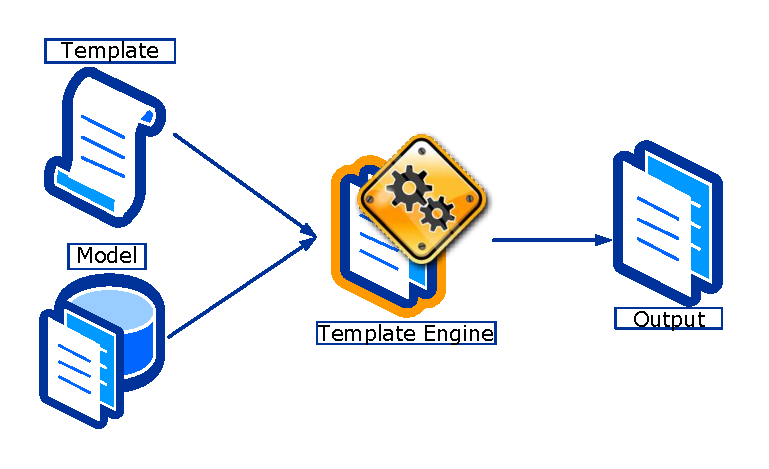
\includegraphics[scale=0.8]{images/TemplateGeneration.pdf}}
    \caption[Template engine]{Figure shows a conceptual view of a template engine.}
    \label{fig:template_engine}
\end{figure}
Figure~\ref{fig:template_engine} depicts the idea behind a template engine. You have some kind of data source (e.g. a model) which get matched towards a template that have markers on where to insert data. After the compilation, the engine outputs what is defined in the template.

\subsubsection{JET}
Java Emitter Templates is a template engine in the M2T (model-to-text) project within the Eclipse ecosystem. JET provides a well known syntax based on JSP, which  has a standard tag library included, that can be extended with custom tag libraries. It comes with editor support and integration with the Eclipse UI.

\lstset{caption=Simple example showing the JSP like syntax in JET,label=list:jetexample,captionpos=b}
\begin{table}[htbp]
  \centering
\begin{lstlisting}[showstringspaces=false]
<%@ jet package="generator.dpf"
  class="DpfGen" 
  imports ="generator.dpf.blog.Article no.hib.dpf.core;"
%>
<% Article art = (Article)argument;%>
public class <%=art.getName()%> {
    public <%=art.getName()%>() {

    }
}
\end{lstlisting}
\end{table}

Listing \ref{list:jetexample} shows a very basic example on how a JET file could look like. We also see that objects are used directly, and not interpreted as the generator frameworks.

\subsubsection{Apache Velocity}
Velocity shares a lot of the same properties that JET possesses. The main difference is the template language, where Velocity provides its own. The language is simple, yet powerful, and provides the same functionality that JET can offer. If the standard functionality is not enough, there are sub-projects like VelocityTools that solves problems like date and number formatting, math operations and more. There is a strong focus on separating code from the templates, thus enforcing patterns like MVC. There is no editor support for Eclipse out of the box, this is achieved using third party plug-ins. 

\lstset{language=HTML,caption=Example showing the Velocity template language,label=list:velocityexample,captionpos=b}
\begin{table}[ht]
  \centering
\begin{lstlisting}[showstringspaces=false]
<HTML>
<BODY>
Hello $customer.Name!
<table>
#foreach( $mud in $mudsOnSpecial )
   #if ( $customer.hasPurchased($mud) )
      <tr>
        <td>
          $flogger.getPromo( $mud )
        </td>
      </tr>
   #end
#end
</table>
\end{lstlisting}
\end{table}

\subsection{Code Generation Frameworks}
A code generation framework is more than a simple template engine. The biggest difference lies with the additional tooling around the engine, like debugging, editor support and profiling of templates. The problem identified in section~\ref{sec:metamodels_and_cg} is addressed in these tools through a built-in interpreter which interprets the DSML, and creates a template editing environment where the editor support reflects the domain concepts of the DSML.

\subsubsection{Acceleo}\label{subsec:acceleo}
Acceleo~\cite{acceleo} is the product of Obeo, the same company that is behind Obeo Designer. The project has been in development 
since 2006, and was incorporated into the Eclipse M2T project in 2009. Acceleo is the reference implementation of 
Object Management Group's MOF model to text transformation language (MOFM2T)~\cite{MOFM2T}. It has full integration with EMF, 
which means you can use Ecore, UML2, etc. The framework has support for debugging and profiling templates, as well 
as editor support with auto completion and content assist. The debugger has its own Eclipse view where you can debug the templates directly using breakpoints. You can also step over/into/return functions like Eclipse JDT provides for Java. 

Another notable feature is the generator module system. A generator module is a plug-in with pre-defined generator templates for a particular domain. This enables the users of Acceleo to take advantage of available generators for popular domains. The drawback of this system is that the generators are (of course) bound to a specific type of metamodel, and might not be tailored to the specified requirements.

\lstset{caption=Example showing the MOFM2T language used in Acceleo,label=list:acceleoexample,captionpos=b}
\begin{table}[ht]
  \centering
\begin{lstlisting}[showstringspaces=false]
[template public generate(aClass : Class)]
  [file (aClass.name.concat('.java'), false)]
    public class [aClass.name.toUpperFirst()/] {
    [for (p: Property | aClass.attribute) separator('\n')]
      private [p.type.name/] [p.name/];
    [/for]
  [/file]
[/template]
\end{lstlisting}
\end{table}

\subsubsection{Xpand}
Xpand~\cite{xpand} is a framework under the Eclipse M2T project that facilitates MDE activities such as code generation, model validation and model transformations. The company behind Xpand is Itemis~\cite{itemis}, a german consulting company focusing on utilizing MDE in projects. Xpand has a wide variety of features which makes it a good fit for this projects requirements. Most notably, you can create editors (with code completion and syntax highlighting) from metamodels specified in EMF Ecore, UML2, XSD and JavaBeans. Besides the predefined metamodels, it is possible to define a custom metamodel that is based on an arbitrary modelling language. Xpand is discussed in detail in section~\ref{sec:xpand}\newline

\subsubsection{Comparison}
Table \ref{tab:gen_features} gives an overview of the different features in the evaluated solutions: 
\begin{description}
  \item[Template Language] The language used in the templates.
  \item[Editor Support] All the considered solutions provide some kind of editor support with syntax highlighting and template validation. The difference from the template engines to generator frameworks lies with how this editor support is provided. Xpand and Acceleo interprets the input models and provide an environment for creating templates, extensions and validation based on the metamodel. In a DPF context this means you operate on the concepts of the DSML, rather than the instance model's actual Java objects. This is discussed in detail in section \ref{sec:xpand}.
  \item[Custom Metamodel] Xpand and Acceleo provide support for EMF and UML models out of the box. This means an UML model will act as a metamodel, i.e. expose its domain concepts in the editor environment. This is discussed in detail in section \ref{sec:xpand}.
  \item[Profiler/Debugger] Profilers are used to optimize your templates and extensions, and gives an overview of which parts of the system that is slow. Both Acceleo and Xpand has a profiler.
  A debugger is useful for finding bugs inside the templates. Acceleo allows you to debug templates like Java classes in Eclipse, with a debug view, breakpoints and stepping over/into/return functions.
\end{description}
\let\Oldarraystretch\arraystretch
\renewcommand*\arraystretch{1.5}

\begin{table}[htb]  
  \centering
  \resizebox{1\textwidth}{!}{
    \begin{tabular}{|p{32mm}|p{22mm}|p{27mm}|p{27mm}|p{27mm}|}
      \hline
      \textbf{Tool}                   & \textbf{Template\newline Language}  & \textbf{Editor Support}  & \textbf{Custom\newline Metamodel} & \textbf{Profiler/\newline Debugger}\\
      \hline
      \textbf{Apache Velocity}       & VTL                   & No                                       & No                      & No \\
      \hline
      \textbf{Eclipse JET}           & JSP                   & No                                       & No                      & No \\
      \hline
      \hline
      \textbf{Acceleo}               & MOFM2T                & Yes                                      & No                      & Yes \\
      \hline
      \textbf{Xpand}                 & Xpand                 & Yes                                      & Yes                     & No \\
      \hline
    \end{tabular}
  }
  \caption {Feature comparison in template engines}
  \label{tab:gen_features}
\end{table}
% template language, profiler, template editor, custom generator metamodel, 
\let\arraystretch\Oldarraystretch
The reason for choosing Xpand is together with the rich tooling, the possibility of creating a custom metamodel. The included profiler is a welcomed feature, but was not critical to the choice of solution. The choice of template language was not crucial either, but a language with its foundation in a standard is a positive trait. Acceleo is providing the same functionality as Xpand with some minor differences in the tooling. A simpler choice would have been either JET or Velocity, but this would be a poor solution for the end-users because of the lack of tooling. Both Acceleo and Xpand provides a "sandboxed" editor environment, which means the template coder only has access to the DSML concepts which is defined through a Xpand/Acceleo metamodel.

\section{Xpand}\label{sec:xpand}
% OAW og naming
Xpand is created and maintained by the german consulting company Itemis~\cite{itemis}. Before the project was included into the Eclipse M2T project, it was called \emph{openArchitectureware (oAW)}~\cite{OAW08Manual}. The functionality is the same, but the project has been split up into different Eclipse projects. Xpand is under the M2T project, while the \emph{Modeling Workflow Engine (MWE)} is under \emph{Eclipse Modeling Framework Technology (EMFT)}. The workflow engine connects the different components in Xpand and executes them. Even though the components have a clear separation, we will use Xpand for all of the included technologies, and explain them when needed.

The biggest difference from a simple template engine, is the built-in interpreter that interprets a DSML and provides functionality based on what a Xpand metamodel dictates. In Xpand, the metamodel is the internal mapping from types in the DSML to types that Xpand understands. Xpand comes with metamodels for the most popular modelling facilities today; EMF, UML2, XSD and plain Java classes. Although these metamodels covers the most used languages, it lacks support for DSMLs specified in anything besides what Xpand has to offer. There are a lot of proprietary DSMLs out there which is not modeled in any of the mentioned languages. Acceleo solves this by saying you need to specify your DSML in EMF/EMOF. This is not a generic solution, and requires the users to create a new EMF/EMOF implementation for each new language that is created. A solution to this problem is to create a model-to-model transformation which can transform your DSML to EMF. The disadvantage is that you are still restricted to the functionality that the Acceleo metamodel defines (which is the EMF concepts), when you perhaps would want to define your own.

DPF is a framework for creating DSMLs, and as discussed in chapter \ref{chap:model_based_development}, DPF Editor falls under the language workbench category. The use case for the DPF project is to generate tooling based on a specified DSML; we want a generic way to define generators for an arbitrary DSML. This use case is a bit narrow, and is probably why Acceleo has not facilitated custom metamodels. Xpand fits our criteria nicely with the ability to create custom metamodels with custom attributes and operations. Xpand lets us create a separate API used only in the templates and extensions, on top of the existing functionality that resides in the DPF Core API. The metamodel defines a mapping from DPF types to Xpand types which is reflected in the template/extension editor. 

Xpand is a feature rich framework with features as \emph{aspect-oriented programming (AOP)}, functional extensions, model-to-model transformations, model-to-text transformations and model validation. The framework provides three different languages that has separate functionality; Xpand, Xtend and Check.
% Noko om namnet
% Må eg sei at metamodel betyr Xpand metamodel?
% javabeans er internal
\begin{description}
  \item[Xpand] \hfill \\
    Xpand is the template language that controls the output of the generator. Apart from the usual control flow statements, it supports lazy evaluation, \codeText{let} statements, aspect oriented programming and extensions created using Xtend and/or Java.
\newpage
\lstset{caption=Example showing the Xpand syntax,label=list:xpandexample,captionpos=b}
% \begin{table}[ht]
%   \centering
  \begin{lstlisting}[showstringspaces=false]
«IMPORT dpf
«EXTENSION org::eclipse::xtend::util::stdlib::io»
 
«DEFINE main FOR dpf::Specification»
  «EXPAND graph FOR this.graph»
«ENDDEFINE»
 
«DEFINE graph FOR dpf::Graph»
  «EXPAND domainclasses FOREACH this.getDomainClasses()»
«ENDDEFINE»
 
«DEFINE domainclasses FOR dpf::DomainClass»
  «syserr(this.name)»
«ENDDEFINE»
  \end{lstlisting}
% \end{table}
    This listing shows a simple template where we traverse our DPF Specification and print out the name of a DSML type called \emph{DomainClass}. We also see how the inclusion of extensions are performed. These extensions are defined in Xtend and/or Java.
  
  \item[Xtend] \hfill \\
    Xtend is used as an extension language. It follows the functional paradigm and provides features like type inference, recursion, caching of methods and calling external Java extensions. It also provides ways to perform model-to-model transformations. This language helps to enforce the separation between program logic and template code; it is strongly encouraged to perform logic in an extension, and call the extension from the template. Such extensions are called \emph{embedment helpers}~\cite{fowler2010domain}.
\lstset{caption=Example showing Xtend extensions,label=list:xtendexample,captionpos=b}
% \begin{table}[ht]
%   \centering  
  \begin{lstlisting}[showstringspaces=false]
importDate(dpf::DomainClass this) :
  if this.getAAttributes().exists(e | e.target.name == "Date") then
	"import java.util.Date;";

String paramList(List[dpf::DomainClass] this) :
  JAVA no.hib.dpf.codegen.generator.extensions.
	StringUtil.getAttributeList(java.util.List);
  \end{lstlisting}
% \end{table}
    Listing~\ref{list:xtendexample} shows the Xtend language, with two Xtend methods. \codeText{importDate} shows how we detect a \emph{Date} type defined in our DPF model. If such a type exists, we return a string that contains an import statement. This example demonstrates the type inference by not declaring a return value. It also showcases some of the functional syntax with the \codeText{exists} statement, which returns a boolean value based on the expression within.
    The last example shows how a Java extension is called from Xtend. Type inference from these extensions are not supported, so we explicitly need to declare the return type. We also observe the need to use fully qualified method names for the extension class. This method in particular returns a \codeText{String} that has been constructed from a list of \codeText{DomainClass} types.
% Reducing \emph{foreign code} in the templates improves readability drastically. 
  \item[Check] \hfill \\
    The Check language handles constraint checking on the model.
\lstset{caption=Example showing a simple constraint check,label=list:checkexample,captionpos=b}
% \begin{table}[ht]
%   \centering  
  \begin{lstlisting}[showstringspaces=false]
import dpf;

context Attribute ERROR
  "Name of " + name + "too short." : name.length > 1;
  \end{lstlisting}
% \end{table}
    Listing \ref{list:checkexample} shows a simple constraint check. The first line imports the metamodel. The second and third line checks the length of property \emph{name} in \codeText{Attribute}, and returns an \codeText{ERROR} if the test fails. Denoting the Check statement with \codeText{ERROR} will abort the workflow and print the error to a console. Alternatively, one can use \codeText{WARNING}, which will print the warning and continue the workflow.
    In the DPF Editor the constraint checking is done within the DPF model, but all validation could happen in the generation phase using Check if desired.
\end{description}
These languages are built upon the same type system, and share a lot of the syntax. The shared syntax is called the \emph{expression sub-language} and provides the basic flow control constructs of all the three languages (e.g. if-conditions, switch statements, casting). The expression sub-language syntax is a mix between Java and OCL.

\subsubsection{Workflow}\label{subsub:workflow}
The Modeling Workflow Engine (MWE) provides a way to execute different Eclipse modelling components in a sequential manner. The execution environment can be inside Eclipse or standalone. Modelling components do not have to be part of the Xpand framework; a component needs to adhere to an interface which MWE provides.

A workflow is defined in a XML file, where each component has its own configuration. Some of the components in Xpand are shown in listing \ref{list:workflowexample}. A workflow do not have to include all of the components shown; a typical workflow for generating code only consists of a reader and generator component.
\newpage
\lstset{language=XML,caption=An example MWE workflow file,label=list:workflowexample,captionpos=b,breaklines=true}
\begin{table}[htpb]
  \centering  
  \begin{lstlisting}[showstringspaces=false]
    <?xml version="1.0"?>
    <workflow>
(1)	    <property name="model" value="path/to/model/Model.xmi" />
	    <property name="src-gen" value="src-gen" />
	    
(2)	    <bean class="org.eclipse.emf.mwe.utils.StandaloneSetup" >
		    <platformUri value=".."/>
	    </bean>
	    
(3)	    <bean id="mm_emf" class="org.eclipse.xtend.typesystem.emf.EmfRegistryMetaModel"/>

(4)	    <component class="org.eclipse.emf.mwe.utils.Reader">
		    <uri value="platform:/resource/${model}" />
		    <modelSlot value="model" />
	    </component>

(5)	    <component class="org.eclipse.xtend.check.CheckComponent">
		    <metaModel idRef="mm_emf"/>
		    <checkFile value="metamodel::Checks" />
		    <emfAllChildrenSlot value="model" />
	    </component>

(6)	    <component class="org.eclipse.xtend.XtendComponent">
		    <metaModel class="org.eclipse.xtend.typesystem.emf.EmfRegistryMetaModel">
			  <metaModelFile value="${model}"/>
		    </metaModel>
		    <invoke value="test::Trafo::duplicate(rootElement)"/>
		    <outputSlot value="newModel"/>
	    </component>

(7)	    <component class="org.eclipse.xpand2.Generator">
		    <metaModel idRef="mm_emf"/>
		    <expand
			    value="template::Template::main FOR model" />
		    <outlet path="${src-gen}" >
			    <postprocessor class="org.eclipse.xpand2.output.JavaBeautifier" />
		    </outlet>
	    </component>
    </workflow>
  \end{lstlisting}
\end{table}

Listing \ref{list:workflowexample} shows a workflow file where an Ecore model is used for input:
\begin{enumerate}
  \item The first lines declares properties for model location and the output folder for the results.
  \item \codeText{StandaloneSetup} is used to initiate EMF specific functionality, like \codeText{platform:/resource} URIs.
  \item Initiation of the Xpand metamodel. The handle \codeText{mm\_emf} is used to refer the metamodel throughout the workflow definition.
  \item The \codeText{Reader} component is used to read the input model's Ecore, and then create a \emph{slot} which stores the model in a named attribute.
  \item This is the configuration of the \codeText{Check} component. We define the EMF metamodel to operate on, as well as the name of the Check file.
  \item The \codeText{Xtend} component performs a model-to-model transformation based on the rules specified in the Xtend file.
  \item The generator component is the one generating code. We start off by defining the EMF metamodel, then we define the entry point in the templates, and also refer the model that the template should be run on. Finally, we define an outlet path where the resulting code should be written to. We also apply a postprocessor to our output, in this case a \codeText{JavaBeautifier}. The \codeText{JavaBeautifier} is a class which format the generator output to our needs. There are postprocessors included in Xpand for C++, Java and XML.
\end{enumerate} 

It is important to point out that the order of the components matter. Before using a Xpand metamodel it is necessary to use its corresponding reader component first (if it has one). Using a metamodel dependent component with an uninitalized metamodel will result in errors.

\begin{figure}[htpb]
  \centering
  \centerline{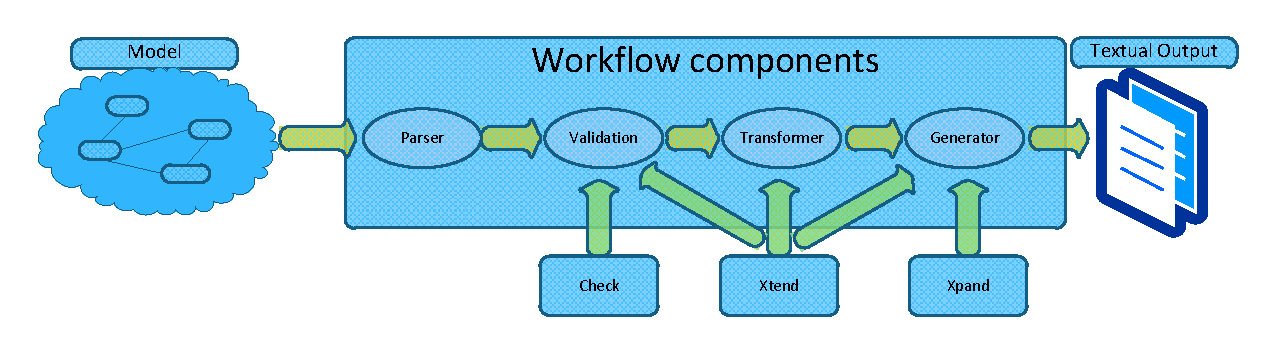
\includegraphics[scale=0.8]{images/xpandworkflow.pdf}}
  \caption[Workflow in Xpand]{Figure shows how the workflow engine works.}
  \label{fig:xpand_workflow}
\end{figure}

Figure \ref{fig:xpand_workflow} depicts a workflow in Xpand. Although a usual workflow, all of the components are optional, and could be replaced by something else.
\newpage
\subsection{Xtend 2}\label{subsec:xtend2}
In December 2011, version 2.2 of Xtend~\cite{xtend2} was released. This is Xpand's successor, and is the main focus for Itemis from now on.  Xpand will be maintained for a while, but will probably be dropped in favour of Xtend 2 in the longterm. 

The naming is a bit confusing, as the Xpand framework has a separate language called Xtend (see listing \ref{list:xtendexample}). Xtend 2 is a complete rewrite and is not compatible with older versions of Xpand. It is based on Xtext~\cite{xtext}, another Eclipse project created by Itemis. Xtext is a language workbench for textual languages where one can create editors and generators from a grammar. Currently Xtend 2 is a part of the Xtext project, but will in time become a separate project. The reason for this re-implementation is mentioned in the lead developer Sven Efftinge's blog~\cite{efftinge_blog}; performance issues, poor tooling and shortcuts in the language.

Xtend 2 is a fully-fledged programming language, which compiles to readable Java code. The language aims to reduce the verbosity of Java, and support features like type inference, closures and operator overloading. Generating code is done through what is called \emph{template expressions}, which is the syntax from Xpand embedded into the Xtend 2 language. Instead of the interpreter based approach of Xpand, the template expressions are compiled to Java code. At the time of writing, Xtend 2 do not provide the same functionality as Xpand as it has no support for loading custom models.

Xtend 2 can work on a grammar defined in Xtext, which in its turn has its foundation in EMF Ecore. More information on this works can be found in the Xtext/Xtend documentation~\cite{xtend_codegen}. Further information on Xtend 2 can be found at Xtend web site, and Sven Efftinge's blog as well ~\cite{xtend2}~\cite{efftinge_blog}.

% Det er mogleg med interpreters i xtext
% Lage figur som viser korleis ein får editor support frå Xpand metamodel
% http://www.eclipse.org/forums/index.php/m/798256/#msg_798256
%     \item Xpand successor: http://blog.efftinge.de/2010/12/xtend-2-successor-to-xpand.html
%     \item Xpand artiklar: http://blog.efftinge.de/search?q=xpand
% http://www.eclipse.org/Xtext/documentation/2_0_0/040-first-code-generator.php
% http://www.eclipse.org/Xtext/documentation/2_0_0/210-emf-integration.php#emf_codegen
% Xpand interpreted
% Xtend compiled